% chktex-file 1
% chktex-file 46
\section{Reviewer \#1}\label{reviewer_1}

\subsection*{Overall comments}

\RC{} This study proposed an integrated index that incorporates water resources, water use, and water allocation to represent the water governance regime in the Yellow River basin. The authors showed an in-depth understanding of the water governance in this basin and made a great effort to represent the status of water governance straightforwardly with the integrated index. The figures were generally well-designed and presented clearly. But I feel the paper lacks details of the results which makes it difficult to understand the paper. Specific comments are listed below.

% 感谢您认可。
% 很抱歉缺少细节,可能会使您难以完全理解我们的研究。
% 为了回应您的担忧,我们已经修改了我们的稿件,并提供了更详细的结果解释。请在下面找到我们对您的具体评论的逐条回复。
\AR{} Thank you for your valuable feedback and for acknowledging our efforts in understanding the water governance in the Yellow River basin. We appreciate your comments regarding the clarity of the figures and our integrated index. Sorry about the lack of details in the results section may have made it difficult to fully comprehend our study. In response to your concerns, we have revised our manuscript and provided a more detailed explanation of the results. Please find our point-by-point response to your specific comments below.

\subsection{Major concern \#1}

% 气候变化在指数中没有明确的体现,这可能是本世纪黄河流量恢复的关键因素。气候变化将是未来该流域面临的巨大挑战。重大的气候变化可能影响流域的适应能力,因此需要不同的治理策略。
\RC{} Climate change is not explicitly represented in the index, which might play a key role in the streamflow recovery in the Yellow River in this century. Climate change would be a great challenge in the basin in the future. Significant climate change may affect the adaptive capacity of a basin and thus require different governance strategies.

% 气候变化的确会产生很多影响,例如改变降水量和蒸发量。但这些影响都会以影响可用水量的形式体现在IWGI之中。
% 在新增加的图表中,我增加了天然水量的图表展示这种变化
% 例如气候变化让可用水量发生改变(scarcity),极端气候让我们难以有效的分配水资源(allocation),对气候变化的适应可能导致社会变革,让人们对愈发侧重于工业和经济发展的治理策略进行反思(purpose)。
% 我们现在在讨论中涉及了这些话题。
\AR{} Thanks for the comment that we lacked a discussion of climate change, which has a multitude of impacts e.g., on precipitation and evaporation.
However, these effects are inherently captured within the Integrated Water Governance Index (IWGI) because the available water resources are affected by climate change as consequences.
For clarity, we first modified our expression of SFV-index, which is the indicator highly related to climate change (both in water yield and its fluctuation):

\begin{quote}[page=3, sline=78, eline=82]
	The impetus for developing this new index lies in the evolving practices of water governance driven by a blend of social and natural influences.
	Firstly, climate change impacts on current water yield, coupled with escalating demands from economic activities and the need for water storage development, intensify water stress~\cite{qin2019,wada2014,huang2021}.
\end{quote}

\begin{quote}[page=5, sline=144, eline=149]
	We used the scarcity-flexibility-variability (SFV) water stress index proposed by \citeA{qin2019} to evaluate water stress.
	This indicator integrates the share of runoff being consumed, the share of consumption in these inflexible categories and the historical variability of runoff weighted by storage capacity~\cite{qin2019}, where impacts from both management measures and climate changes are included.
	% 这个指数得到了许多应用,是就我们已知范围内考虑因素最为齐全的,反应水资源压力的指数。
	The SFV-index, which has many applications, is the most comprehensive index of water stress we know.
\end{quote}

\AR*{} In addition, we added a new graph (Figure~\ref{fig:runoff}~a) in the revised version of Supporting Information to demonstrate the changes in runoff. Trend of natural runoff can also be inferred from the measured runoff (Figure~\ref{fig:runoff} from b to d) and water use (Figure~\ref{fig:runoff} from e to g). We quote this figure when discussing climate context, now:

\begin{figure}[!ht]
	\centering
	\renewcommand{\thefigure}{S2}
	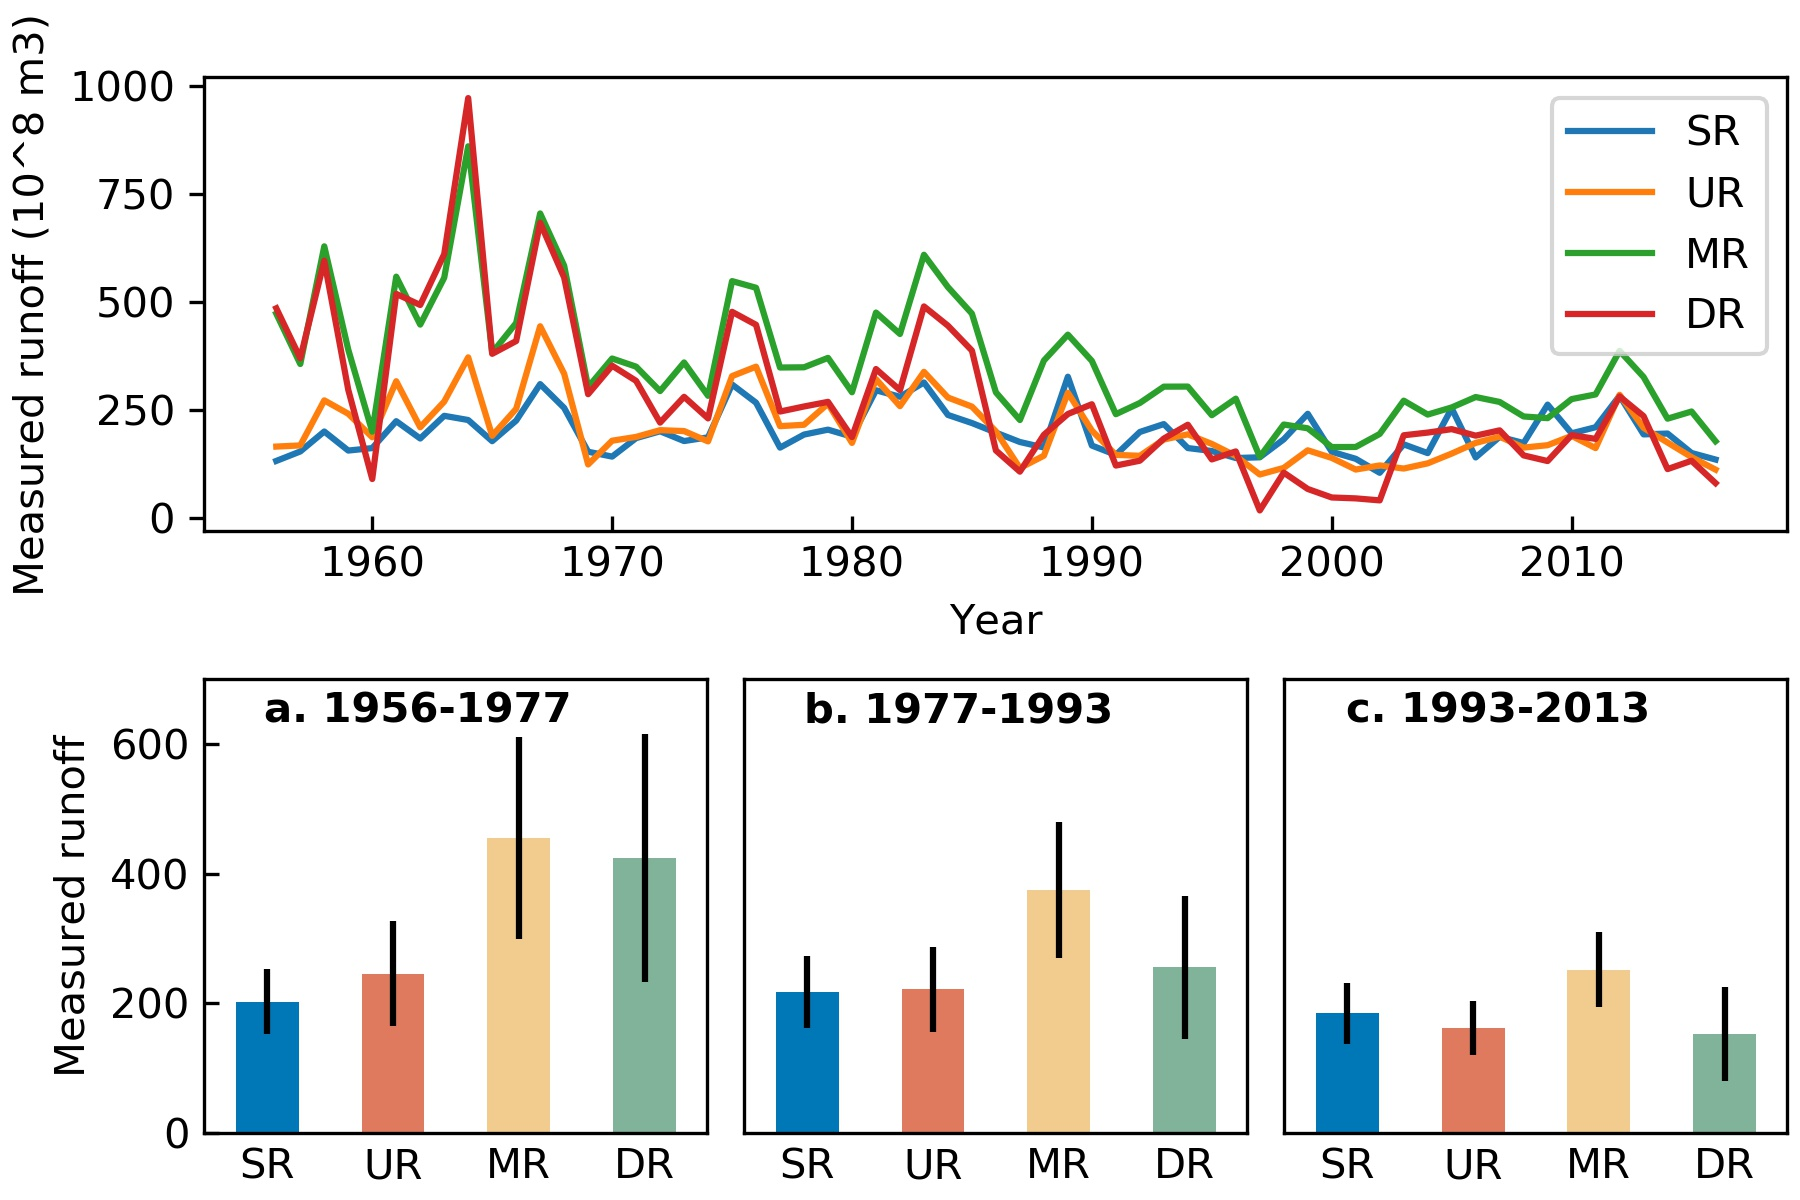
\includegraphics[width=\textwidth]{sup/sf_measured_runoff.jpg}
	\caption{
		\textbf{a.} Measured runoff of different regions in the Yellow River Basin from 1965 to 2013.
		\textbf{b.} Measured runoff of different regions under different water governance regimes.
		\textbf{c.} Natural river runoff of different regions under different water governance regimes.
	}\label{fig:runoff}
\end{figure}

\begin{quote}[page=10, sline=274, eline=277]
	% 一个基本背景是,在用水量总体保持稳定的情况下,黄河流域的径流量已显著低于从前,这是该时期水资源压力重新上升的重要原因。
	Partially because of changed climate~\cite{han2023,liu2020c}, the runoff of the YRB was significantly lower than before when the overall water uses remained stable, which was an important reason for the rise of water stress in this stage (Supporting Informations Figure~\ref{fig:runoff} and Figure~\ref{fig:scarcity}).
\end{quote}

\AR*{} Finally, we further discussed the challenges brought by climate changes in the discussion section:

% 我们强调流域治理需要考虑这些因素,但我们可能很难穷尽优秀的流域治理策略需要考虑哪些因素。因此,IWGI至少让我们可以知道在诸多治理因素的共同影响下,流域的未来正在走向何方。
\begin{quote}[page=11, sline=306, eline=316]
	Future's tightly intertwined socio-hydro interactions can lead water governance challenges even more complex and comprehensive, combining resources issues and structural barriers~\cite{huggins2022a}.
	For example, climate change may alter water scarcity levels and make it more difficult to effectively use water due to extreme climate events, strengthening water stress and threatening infrastructures~\cite{liu2017, dibaldassarre2019}.
	Additionally, adapting to climate change could lead to transformations~\cite{sachs2019,barnes2020}, prompting a reevaluation of governance strategies of social water usage (purpose and allocation) which is being increasingly altered by current regime transitions.
	It may be difficult to exhaust what is considered in a good watershed governance strategy, but the IWGI at least gives us a sense of where the a river basin is heading and how challenged.
\end{quote}

\subsection{Major concern \#2}\label{sec:1-2}
% 结果是总结性的。我建议提供更多关于三个指数和IWGI结果的信息。例如,三个指标的结果,以及分区域的结果。请解释IS、IP、IA和IWGI这三个指标的范围,以及不同数值的含义。这些细节可以帮助读者理解结果的合理性。
\RC{} The results are summative. I would suggest providing more information on the results of the three indices and the IWGI.\ For example, the results of the three indices, and the results for the sub-regions. And please explain the range of the three indicators, IS, IP, IA, and the IWGI, and the meanings of different values. These details could help readers understand the reasonability of the results.

% 感谢您指出这一点,非常抱歉过于总结性的手稿带来的困惑。
% 在新的手稿中,我们将各指数的情况总结到补充材料,并在正文中对有关各指数情况的图表总结。
% 在方法中,我们补充了指标的取值范围(三个子指标的变化范围都是0~1)。
\AR{} Thank you for pointing this out, and we apologize for the confusion caused by the overly conclusive manuscript. In the revised manuscript, we have summarized the indicators by graphs with description in Supporting Information:in the Supporting Information.

\AR*{} Figure~S3, Figure~S4, and Figure~S5 are three indicators changing trends. We added them into Supporting Informations with descriptions:

\begin{figure}[!htb]
	\centering
	\renewcommand{\thefigure}{S5}
	\includegraphics[width=\textwidth]{sup/scarcity.png}
	\caption{Changing trend of the indicator of stress}\label{fig:scarcity}
\end{figure}

\begin{quote}[page=Supporting Informations]
	The index of stress (SFV indicator, IS) in the study period (including three different periods) showed a change trend of first decreasing, then rapidly increasing, and finally slightly decreasing again (Figure~\ref{fig:scarcity}~A), indicating that water resource pressure first decreased, then rapidly increased, and then stabilized.
	Among the four different regions (Figure~\ref{fig:scarcity}~B), the source region (SR) has almost no contribution to IS changes in the three periods, and the downstream region (DR) only has a weak negative contribution in the governance transforming regime and the adaptation oriented regime.
	The upper and middle reaches (UR and MR) had the greatest impact on the IS changes. Wherein, the upper region (UR) made the greatest contribution during the massive supply regime and governance transforming regime, while the middle reaches made the greatest contribution in adaptation oriented regime.
\end{quote}

\begin{figure}[!htb]
	\centering
	\renewcommand{\thefigure}{S3}
	\includegraphics[width=\textwidth]{sup/priority.jpg}
	\caption{Changing trend of the indicator of purpose}\label{fig:purpose}
\end{figure}

\begin{quote}[page=Supporting Informations]
	In terms of water use purpose indicator, IP remained basically unchanged in a massive supply regime, but showed a rapid decline in the period of governance transformation and adaptation oriented regime (Figure~\ref{fig:purpose}~A).
	Throughout the three periods, the change of irrigation water dominated the change of the IP, while urban and rural water for human settlements and rural livestock had almost no influence on the change of IP (Figure~\ref{fig:purpose}).
\end{quote}

\begin{figure}[!htb]
	\centering
	\renewcommand{\thefigure}{S4}
	\includegraphics[width=0.7\textwidth]{sup/allocation.png}
	\caption{Changing trend of the indicator of allocation}\label{fig:allocation}
\end{figure}

\begin{quote}[page=Supporting Informations]
	The water allocation (IA) showed an obvious ``V-shaped'' trend, indicating that water resources in the different regions within the YRB first gradually moved away from uniform distribution, and then gradually tended to uniform distribution since 2000 (Figure~\ref{fig:allocation}).
\end{quote}

\AR*{} In addition, ranges of three indicators and meaning of their values are further explained in the methodology section of main text, now:

\begin{quote}[page=5, sline=137, eline=138]
	where $I'_x$ is calculated by Min-Max normalization of $I_x$ (thus ranges from zero to one):
	\begin{equation}
		I'_x = (I_x - I_{x, \min}) / (I_{x, \max} - I_{x, \min})
	\end{equation}
\end{quote}

\subsection{Major concern \#3}\label{sec:1-3}
% 本研究中使用的数据似乎有不同的时间段,大多数数据来自2013年之前。近十年来,黄河的水文状况和水治理应该发生了重大变化。因此,结合近十年的结果将使这项研究更加可靠。
\RC{} The data used in this study seem to have different time periods, and most data are from before 2013. The hydrological regime and water governance in the Yellow River should have changed significantly in the recent decade. Therefore, incorporating the result from the recent decade would make this study more solid.

% 感谢审稿人的宝贵建议,但出于以下原因,我们无法在新的手稿中将研究时段后延至今
\AR{} Thanks for the reviewer's valuable advice, but for the following reasons, we are unable to postpone the study period to date in the main text. Instead, we added robustness test by using different-source data in Supporting Information.

% 首先,本研究结论希望展现黄河水治理演变过程,尤其是重点关注1978到2001年之间的治理转型过程。尽管许多数据能在近二十年间计算IWGI,但代价是忽略了更远的时间段。而正如我们在新手稿的方法部分所补充说明的,使用不同的数据源容易造成时间不连续的问题(通常它们的统计口径是不一样的)。
\AR*{} Firstly, the conclusion of this study aims to show the evolution process of water governance of the Yellow River, especially focusing on the governance transformation between 1978 and 2001. Although many dataset allow IWGI to be calculated over the last two decades, the cost is to ignore the more important past periods. In addition, it's difficult to assimilate the different data sources because datasets usually have different statistical approach when categorizing water use sectors. Now, we added an explanation in the methods section of the new manuscript:

\begin{quote}[page=5, sline=138, eline=140]
	Since the IWGI essentially comprises by three aspects' indicator with same weights, its prerequisite is to keep the same data source for each indicator throughout time, to ensure time series continuity.
\end{quote}

\AR*{} Secondly, as the reviewer noticed, we used multiple-source dataset to implement our approach, which means time periods of a coherent analysis is limited by the shortest data. To cover study period from 1960s to 2000s, water use data developed by \citeA{zhou2020} is the most good quality and widely used dataset. The shortage, however, is not enough to cover the period after 2013. We contacted the original author team, but only confirmed that latest dataset is still unavailable. As some of the source data used to produce this crucial dataset could not be easily supplemented, this was not an effort that could be supplemented in this study. Therefore, we decided to keep the analysis discontinued in 2013 in main texts:

\begin{quote}[page=11, sline=323, eline=325]
	Another limitation is the lack of latest datasets which is coherent with the historical datasets, so our analysis had to discontinued in 2013 despite potential shifts existing.
\end{quote}

\AR*{} Last, we tried our best to strengthen robustness of this study despite the above limitations. We calculated IWGI by using another data source for the past two decades. Since our results suggest no significant regime change, we think it is robust that the YRB experienced two significant water governance regime changes.

\begin{figure}[!htb]
	\centering
	\renewcommand{\thefigure}{S9}
	\includegraphics[width=0.8\textwidth]{sup/robustness.png}
	\caption{Recent years' IWGI changes}\label{fig:recent}
\end{figure}


\begin{quote}[page=11, sline=325, eline=327]
	As a supplement, we examined IWGI framework with fewer datasets from different source in recent decades where showing no significant regime changes (Supporting Informations~S9).
\end{quote}

\subsection{Major concern \#4}
% 这三个指标之间可能存在相互作用/相互联系。作者是否检查了指标之间的关系?
\RC{} There might be interactions/interconnections among the three indicators. Did the authors examine the relations between the indicators?

\AR{} Yes, we did examination for the interconnections between the three indicators. Sorry we didn't make the information accessible. Now, we added a table to describe this in the Supporting Information (Table~S1).

% Table generated by Excel2LaTeX from sheet '相关性情况'
\begin{table}[htbp]
    \centering
    \caption{The correlation of the Integrated Governance Index (IWGI) and its three sub-indicators (IS, IP, IA)}
      \begin{tabularx}{\textwidth}{XXXXXXX}
      \toprule
      Period & \multicolumn{1}{l}{IS vs IP} & \multicolumn{1}{l}{IS vs IA} & IP vs IA & \multicolumn{1}{l}{IP vs IWGI} & \multicolumn{1}{l}{IA vs IWGI} & \multicolumn{1}{l}{IS vs IWGI} \\
      \midrule
      P1 to P3 & \multicolumn{1}{l}{-0.75 *} & -0.29 & 0.36 & 0.37  & \multicolumn{1}{l}{0.75 *} & 0.14 \\
      P1    & -0.08 & -0.31 & 0.06 & 0.14  & 0.51  & 0.65 \\
      P2    & \multicolumn{1}{l}{-0.90 *} & \multicolumn{1}{l}{-0.87 *} & 0.77 * & -0.18 & -0.13 & 0.5 \\
      P3    & 0     & -0.38 & -0.86 * & -0.33 & 0.61  & 0 \\
      \bottomrule
      \end{tabularx}%
    \label{tab:corr}%
\end{table}%


\begin{quote}[page=Supporting Informations]
	By analyzing the correlation of the integrated management index (IWGI) and its three sub-indexes: stress (IS), purpose (IP) and allocation (IA) in three different periods, namely, the massive supply regime (P1: $1965 \sim 1978$), governance transforming regime (P2: $1979 \sim 2001$) and adaptation oriented regime (P3: $2002 \sim 2013$), the following results are obtained.

	When we focus on the correlation from P1 to P3, the results show significant negative correlation between IS and IP (correlation coefficient is $r = -0.75$, $p < 0.01$), indicating that there is a strong negative relationship between IS and IP.\
	On the other hand, there is a significant positive correlation between IA and IWGI (correlation coefficients are $r = 0.75$, $p < 0.01$), indicating a positive relationship between IA and IWGI.\ However, the correlations of other combinations are not statistically significant overall.

	The correlations between time periods are very different with the overall trend above.
	There is no significant correlation between any indicator combinations in the massive supply regime (P1).
	In the governance transforming regime (P2), there is a significant negative correlation between IS and IP (correlation coefficient $r = -0.90$, $p < 0.01$), a significant negative correlation between IS and IA (correlation coefficient $r = -0.87$, $p < 0.01$), and a significant positive correlation between IP and IA (correlation coefficient $r = 0.77$, $p < 0.01$).
	The correlations between IS and IP, IS and IA, and IS and IWGI were not statistically significant in the adaptation oriented regime (P3). However, there is a significant negative correlation between IP and IA (correlation coefficients are $r = -0.86$, $p < 0.01$).
\end{quote}

\AR*{} In addition, note that strictly independent of indicators is not required in our approach, as three aspects are intertwined in essence (we explained this in the introduction).
% 这是因为,如果两个子指标在某时期内相关性显著,可能说明两者在该时期同时受到某些治理驱动因素的共同作用,这是可能发生的。
This is because a significant correlation between two indicators in a given period may indicate that both were simultaneously affected by some governance drivers during that period, which is possible.
% 但同样,若两个指标始终都存在较强的关联,则可能说明稳态转换并不显著,IWGI同时考虑三者的意义也存疑。
Similarly, if there is always a strong correlation between the two indicators, it may indicate that the steady-state transformation is not significant, and the significance of IWGI considering the three indicators at the same time is doubtful.
% 然而,正如我们在表x中所展示的,IS, IP, IA三者两两之间的关系在不同稳态下都有不同的特征,这佐证了我们IWGI同时考虑三者的意义,以及稳态转换的存在。
However, as we have shown in Table~S1, the relationship between IS, IP and IA has different characteristics under different regimes, which proves that IWGI considers the significance of the three aspects at the same time, as well as the existence of regime shifts.

\subsection{Major concern \#5}
% IWGI在“应力”方面包含储层存储信息。输水能力是衡量水治理/水社会复原力的重要指标。
\RC{} The IWGI includes reservoir storage information in the ``stress'' aspect. However, the water conveyance ability is not represented, which is also an important indicator of water governance/hydrosocial resilience.

% 短期的输水能力是衡量水治理/水社会复原力的重要指标
% 但年尺度上,变化不大
\AR{} We agree that conveyance is crucial to water governance/water society resilience, especially in the short term. However, the IWGI in this study focuses on annual time resolution. At this scale, conveyance has a less significant impact on water governance. From this point of view, there are two reasons that IWGI doesn't have to consider this in our study:

% 输水是水治理的手段,我们更侧重于这种治理的结果。
\AR*{} Firstly, water conveyance is more like an approach of water governance, and we focus more on the outcomes -i.e., how water stress is relieved by conveyance; how it help provision to specific sectors with higher purpose; how convert water changes allocation of water resources \dots

% 水治理很复杂,考虑到越来越多的要素会增加其复杂度。Scarcity是本研究使用最复杂的指标,因为这是一个经过检验的,可以有效表征的指数。如果经过检验影响不大,没有必要增加复杂度。
\AR*{} Secondly, water governance is comprehensive, and taking into account more and more elements increases its complexity. SFV-index is the most complex index used in this study, because it is a tested index that can be effectively represented. If not necessary, we prefer not to include more complexity.

% 我们检验过了年尺度的输水数据,基本变化不大
\AR*{} Finally, since we agree the conveyance is a good view to investigate water governance, we added an examination of the monthly conveyance flow differences of the major reservoirs and their variability in Supporting Information. According to the Yellow River Water Conservancy Commission (YRCC, data source), these reservoirs are mainly for managing and regulating the whole basin. The result (Figure~\ref{fig:conveyance}) shows that variability increased in the later regimes, supporting our main results that regulation plays a more significant role since the governance transforming regime (P2). We also appropriately modified the description in main text:


\begin{figure}[!htb]
	\centering
	\renewcommand{\thefigure}{S8}
	\includegraphics[width=0.8\textwidth]{sup/conveyance.png}
	\caption{Monthly conveyance flow differences of the reservoirs mainly for managing and regulating the whole basin and their variability}\label{fig:conveyance}
\end{figure}

\begin{quote}[page=8, sline=223, eline=225]
	Ensuing the P2, the number of new reservoirs decreased but boosted their role in water regulating and management (more red circles in Figure~3~C, and larger water conveyance variability in Supporting Informations Figure~\ref{fig:conveyance}).
\end{quote}

\subsection{Major concern \#6}
% 我建议在标题中加上“黄河流域”。因为没有对IWGI的适用性和有效性进行测试或讨论。它能在其他盆地使用吗?使用索引的先决条件是什么?
\RC{} I would suggest adding ``Yellow River basin'' in the title. Because the applicability and validity of the IWGI were not tested or discussed. Can it be used in other basins? What is the prerequisite for using the index?

% 感谢你的提议,我们现在在标题中增加了黄河流域,新的标题是:
\AR{} Thanks to your proposal, we have now added the Yellow River Basin to the title, and the new title is: \textbf{``Identifying regime transitions for water governance: Take the Yellow River Basin in China as case''}

% 关于IWGI的泛用性,实际上我们曾在讨论中讨论了这一点。
% 非常抱歉先前的讨论似乎不够明确,我们在修改后的论文中重新澄清了这点。
\AR*{} Regarding the generality of IWGI, we actually discussed this in our discussion. I am very sorry that the previous discussion seems not clear enough, and we have clarified this point again in the revised manuscript.

\begin{quote}[page=11, sline=317, eline=323]
	One of the main limitations in the approach is the lack of multi-sources data in long-term period worldwide, which means there is still a gap between comprehensively identifying and applying the IWGI widely.
	We propose that all water governance issues, however, can change ``who gets water, when and how'' so monitoring such an integrated index is essential, even use simpler indicators.
	We suggest that choices of indicators for different aspects can be adapted according to available datasets -e.g., replace the SFV-index (IA) with simpler scarcity index or proportion-based purpose indicator (IP) by complicated one.
\end{quote}

% 此外,我们如今在方法部分提到了使用它的先决条件,使用同样数据源保证单一子指标的时间序列连贯性,而不同子指标可以采用不同的数据源。
\AR*{} In addition, we have now mentioned in the methods section:

\begin{quote}[page=5, sline=138, eline=142]
	Since the IWGI essentially comprises by three aspects' indicator with same weights, its prerequisite is to keep the same data source for each indicator throughout time, to ensure time series continuity.
	However, vary data sources can be used when estimating the specific indicator or cross different indicators, which makes IWGI a flexible framework for substituted indicators.
\end{quote}

\subsection{Major concern \#7}
% 最好在引言部分解释“水治理机制”的概念,然后解释使用综合指数IWGI代表水治理机制的必要性。
\RC{} It would be better to explain the concept ``water governance regime'' in Introduction and then explain the necessity of using the integrated index IWGI for representing the water governance regime.

% 感谢你的建议,我们在引言部分为“水治理机制”提供了一个简短但明确的解释:
\AR{} Thanks for your advice, we nor provide a short but clear explanation of the ``water governance regime'' in the introduction:

\begin{quote}[page=3, sline=93, eline=98]
	A critical step in understanding the successes and failures of water governance is to identify the different regimes that underpin it~\cite{kjellen2015, grafton2013}.
	Regimes of water governance, the general guidelines of governing practices, arise within linked human-water systems (based on management, institutions, and exploitation) to create local equilibria in social-ecological structures and functions~\cite{falkenmark2021,bressers2013,loch2020,pahl-wostl2007}.
\end{quote}

% 我们还为这种指数的必要性做出了补充:
\AR*{} We also add to the argument for the need for such an index:

\begin{quote}[page=2, sline=66, eline=77]
	Research into index-based water governance assessment generally fall into two categories: those that focus on water systems, and those that concentrate on governance systems.
	On one hand, studies on governance systems typically employ an qualitative assessment to demonstrate what practices influence water governance, e.g., the OECD framework~\cite{oecd2018a}.
	For quantitative studies, due to the lack of comprehensive and detailed information on key components for water governance assessment, these studies often resort to proxy datasets of human activities to create simpler indices~\cite{varis2019,huggins2022a}.
	On the other hand, studies focusing on water systems utilize intuitive indices to encapsulate the outcomes of governance, like the most widely concerned -water stress has been far developed by incorporating human's regulation step by step.
	Specifically, traditional water stress index only demands and supply~\cite{gleick1996}, water scarcity index by involving storage~\cite{damkjaer2017}, and the even more integrated SFV-index includes flexibility~\cite{qin2019}.
	Despite their usefulness, these water stress indices tend not to provide a comprehensive characterization of water governance, as they overlook the social aspect of water usage, i.e., the purpose and allocation of water use.
	As a solution, we propose an integrated water governance index (IWGI) that factors in regional water use allocations and sectoral water use purpose, thereby offering a more comprehensive quantification of governance outcomes.
\end{quote}

\subsection{Detailed issues}

% 我没有在引用的文献中找到“用水的三个核心方面”。这三个方面是作者提出的吗?
\RC{} Line 57$-$62: I did not find the ``three core aspects of water use'' in the cited reference. Were the three aspects put forward by the authors?

% 非常非常感谢您指出这个错误,由于我们弄混了 citation key,这是一个无意间产生的引用错误。
\AR Thank you very, very much for pointing out this error. It was an accidental reference error due to our mix-up of the citation key.

% 总体来说,这是一个引用,但不是逐字逐句的引用,而是基于我们对\citeA{mariajacobson2013}报告的理解。报告在背景部分提出水治理的三个方面,我们将其总结为 stress, purpose, and allocation. 而 what, when, how 的说法则直接来自于该文献,这也是较为广泛的一种对 water governance 如何影响用水的定义。
\AR*{} Overall, this is a quote, but not a word-for-word quote, based on our understanding of a report UNDP participated~\cite{mariajacobson2013}. In the background part of the report, three aspects of water governance are put forward, and we summarize them in as ``stress, purpose, and allocation''. On the other hand, the expression of ``what, when and how'' are directly derived from this literature, which is also a relatively extensive definition of how water governance affects water use~\cite{lasswell2018,allan2001,mariajacobson2013}. Hence, we modified the sentence to:

\begin{quote}[page=2, sline=56, eline=60]
	In this context, the United Nations Development Programme (UNDP) suggests that water governance determines water usage across three core aspects: ``When and what water to use?'' (stress), ``How does water provide different services for human well-being?'' (purpose), and ``Who can use water equally and efficiently?'' (allocation)~\cite{mariajacobson2013}.
\end{quote}

\RC{} Line 92: missing information for the citation?

% 谢谢您指出!再次为我们的粗心感到抱歉
\AR{} Thank you for pointing out! Sorry again for our carelessness. Citations were added in the revised manuscript, now:

\begin{quote}[page=3, sline=108, eline=110]
	Since the 1960s, governance practices such as reservoirs, levees, and conservation measures have contained the issues troubled by thousands of years of high sediment loads~\cite{wang2016a,song2020}.
\end{quote}

\RC{} Line 94$-$95: the sentence is unclear.

\AR{} Sorry about that, we modified that sentence to:

\begin{quote}[page=3, sline=110, eline=113]
	However, new challenges such as decreased streamflows and water depletions occurred in more recent times, followed by different water governance practices like water use regulation and water transfer across basins~\cite{wang2019c}.
\end{quote}

\RC{} Line 121: Repeated citation Qin et al. 2019.

\AR{} Fixed now.

\RC{} Line 122: It would be better to introduce the calculation of SFV in the main text.

\AR{} That's a good suggestion. We now moved the calculation from Supporting Information to the main text.

% 为什么分子W uppro不是W Unon-pro?请核对一下方程式。
\RC{} Equation (6): Why is the numerator WUpro not WUnon-pro? Please check the equation.

\AR{} Thanks for reminding. We used provisioning purpose share in our analysis at last. We forgot to change it's name in texts. We fixed this mistake and everything is coherent now:

\begin{quote}[page=6, sline=157]
	To quantify purpose $I_P$, we used provisioning purpose shares (PPS) of water use as an indicator. While provisioning purpose water use ($WU_{pro}$) includes domestic, irrigated, and livestock water uses, non-provisioning purpose water use ($WU_{non-pro}$) includes industrial and urban services water uses. We calculated the PPS by:
	\begin{equation}
		PPS = \frac{WU_{pro}}{WU_{pro} + WU_{non-pro}}
	\end{equation}
\end{quote}

\RC{} Equation (7): CEM => AEM?\

\AR{} Yep, a typo. We fixed such a stupid mistake now.

\RC{} Line 154: Please explain the source of irrigated area data.

AR{} We cannot dive into every detail of the multi-source datasets in texts, and this dataset is openly published and accessible. Overall, the irrigated area data were obtained by statistical approach in this dataset.

\AR*{} We now attached a new Supporting Information which includes descriptions and all sources of the datasets used in this study. If you want to know more about the data, please check the data source through the provided information.

\RC{} Fig.2A, p<0.01 or p<0.001? (line 147 says that α=0.001 was used for the change-point detection).

\AR{} We used $0.001$ for generating the figure at last (fixed the typo in Fig.2A now). Anyway, as we showed in Supporting Information Figure~S7, no difference in results because the change points are robust.

\RC{} Fig.2C:\ How were the directions determined?

\AR{} We draw the directions for visual convenience. Smaller graph is not for quantitatively illustrating. The arrow of directions are determined by time: point from earlier data to later data locations.

\RC{} Fig.3C:\ What do the dashed lines denote?

\AR{} Sorry about missing necessary description and we now add a sentence in caption of the Fig.3C:\ ``Dashed lines denote average of these percentages in different regimes''.

\RC{} Line 187: what is ``social transformation''?

\AR{} Sorry about the confused expression. I changed the term into ``Social atmosphere'' now. Maybe this is a better phrase.

\RC{} Line 208: the IWGI was proposed in this study, here the citations of Loch's and Turton's studies are not appropriate.

\AR{} The citations should be put at the first half of the sentence, and we fixed this problem now:

\begin{quote}[page=9, sline=238, eline=240]
	The process echoes how societies have been proposed to change governance practices by enhancing their adaptive capacity in the hydrosocial cycle~\cite{loch2020,turton1999}, and the IWGI quantitatively identifies this transition.
\end{quote}

\RC{} Line 273: adapted => adopted?

\AR{} Yep, another typo. We fixed that now.

\RC{} Line 275: biophysical? Please check the sentence.

\AR{} For more clarity, we now changed the sentence to:

\begin{quote}[page=11, sline=330, eline=333]
	In today's world, regime shifts from natural to human-dominated seem likely to become increasingly widespread; comprehensive strategies to address governance challenges will have to become the core of complex human-water systems~\cite{cumming2018,cumming2014,jaeger2019}.
\end{quote}
